\documentclass[../main.tex]{subfiles}
\begin{document}
\chapter{Resultados}
A continuación se presentan los resultados obtenidos mediante la metodología previamente descrita. 

[poner graphical abstract]
\begin{figure}[H]
    \centering
    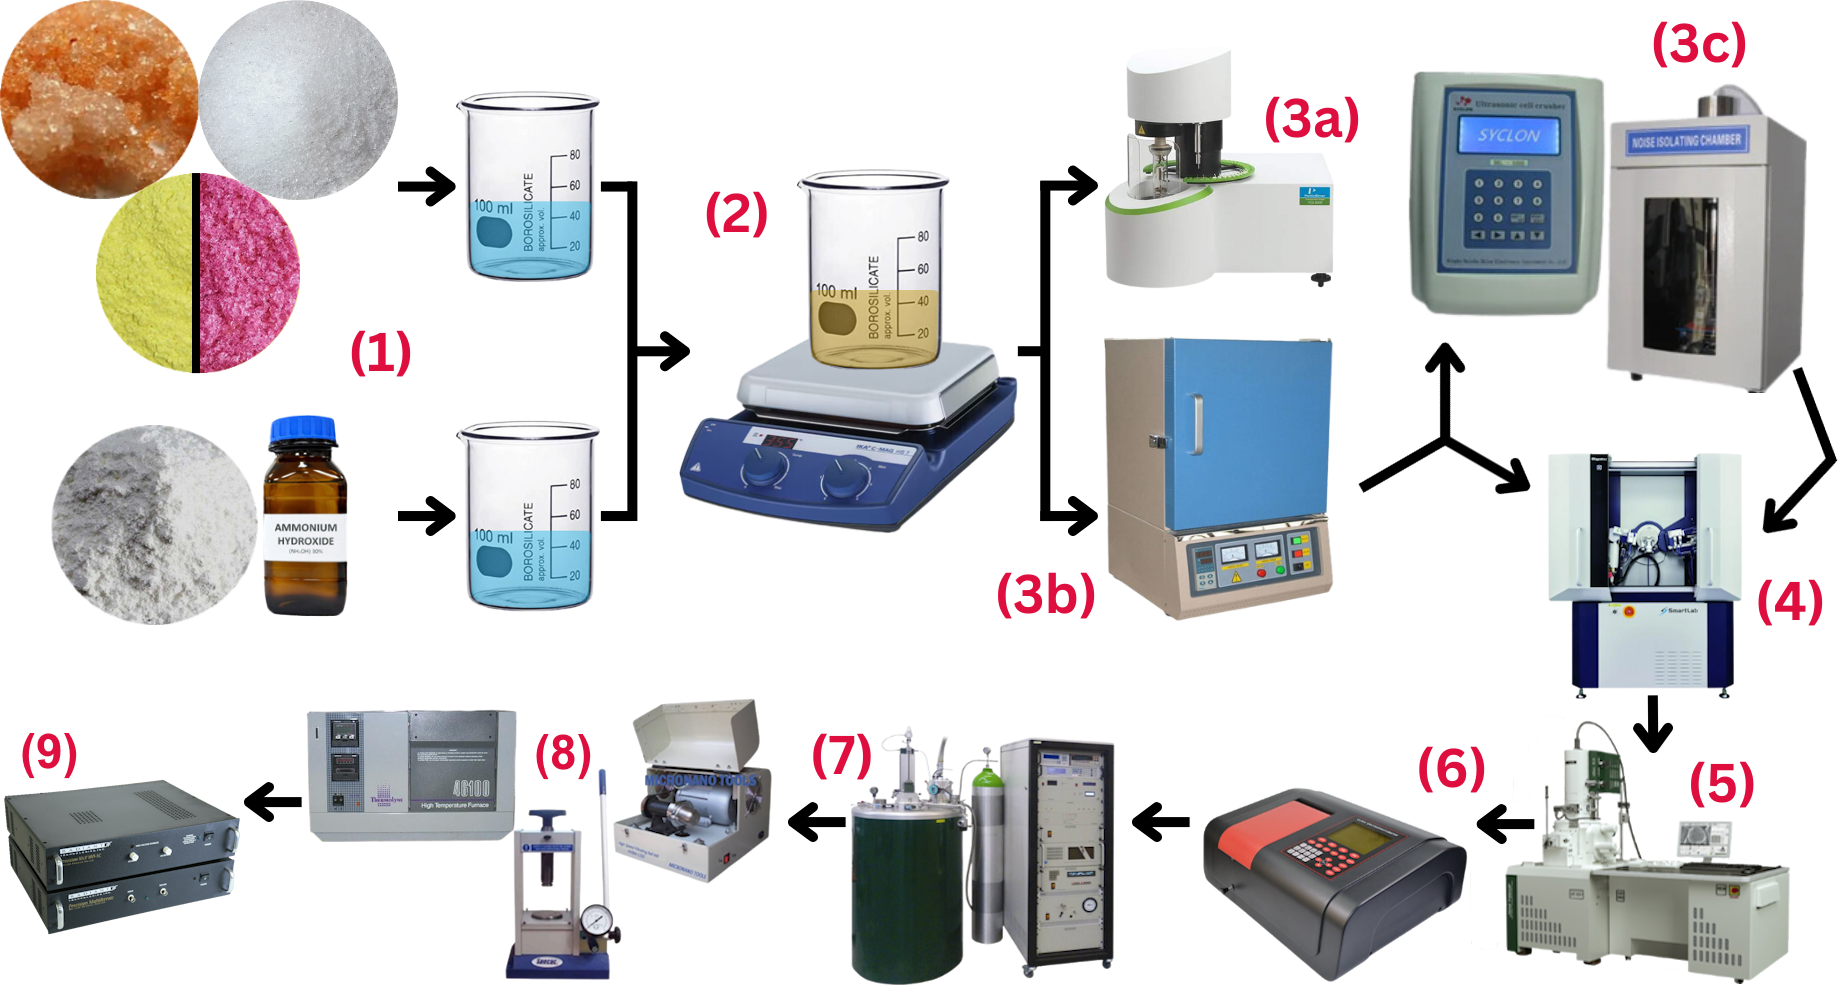
\includegraphics[width=0.7\textwidth]{fig/2.png}
    \caption{Análisis realizados según el equipo utilizado.}
    \label{fig:resdiag}
\end{figure}
\section{Muestras Sintetizadas}

\section{Caracterización}

\subsection{Análisis Termogravimétrico}

\subsection{Difracción de Rayos X}

\subsection{Microscopía Electrónica de Barrido}

\subsubsection{Morfología}

\subsubsection{EDS}

\subsection{Espectroscopía UV-Vis}

\subsection{Magnetometría}

\subsubsection{Dispositivo Superconductor de Interferencia Cuántica}

\paragraph{M vs T}

\paragraph{\textchi{} vs T}

\paragraph{M v H}
\end{document}